\documentclass[10pt]{article}
\usepackage[margin=0.58in]{geometry}
\usepackage{amsmath,amssymb}
\usepackage[T1]{fontenc}
\usepackage{hyperref}
\usepackage{tikz}
\usetikzlibrary{arrows.meta,positioning,fit}
\hypersetup{
  colorlinks=true,
  linkcolor=black,
  citecolor=black,
  urlcolor=blue,
  pdftitle={A Bounded Neuro-Symbolic Loop with EML Trees and qNS Masks},
  pdfauthor={Dana Edwards}
}
\setlength{\parindent}{0pt}
\setlength{\parskip}{2.4pt}
\setlength{\abovedisplayskip}{4pt}
\setlength{\belowdisplayskip}{4pt}
\renewcommand{\baselinestretch}{0.94}
\pagestyle{plain}

\title{\vspace{-1.2em}A Bounded Neuro-Symbolic Loop\\
with EML Trees and qNS Masks\vspace{-0.4em}}
\author{Dana Edwards}
\date{April 20, 2026}

\begin{document}
\maketitle
\vspace{-1.8em}

\begin{abstract}
\noindent
This note records a bounded Tau-adjacent experiment in which a neural or
external proposer emits symbolic formula candidates, a small EML grammar gives
the candidate language, a finite qNS Boolean algebra routes evidence masks, and
Tau checks promotion and table-memory updates over finite audited masks. The
central pattern is
\[
q_{\mathrm{NS}}(y\mid x)
\propto
q_{\mathrm{N}}(y\mid x)\chi_{\mathrm{S}}(y,x),
\]
read as: the neural side proposes and scores, while the symbolic side filters.
The current implementation is not native analytic Tau semantics and not a
general symbolic-regression theorem. It is a certificate-carrying bounded
loop: formula proposal, parse and domain checks, finite sample checks, proof
metadata, qNS mask routing, tamper rejection, and pointwise memory revision.
\end{abstract}
\vspace{-0.5em}

\begin{center}
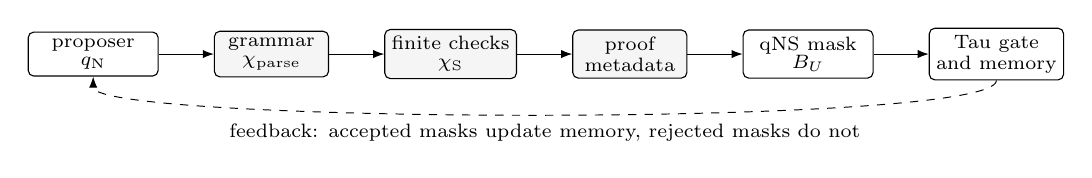
\begin{tikzpicture}[
  node distance=0.55cm and 0.7cm,
  box/.style={draw, rounded corners=2pt, align=center, inner sep=2.5pt,
    minimum width=1.65cm, minimum height=0.55cm, font=\scriptsize},
  gate/.style={draw, rounded corners=2pt, align=center, inner sep=2.5pt,
    minimum width=1.45cm, minimum height=0.55cm, font=\scriptsize, fill=gray!8},
  arrow/.style={-{Latex[length=1.4mm]}, line width=0.35pt},
  note/.style={align=center, font=\scriptsize}
]
\node[box] (prop) {proposer\\[-1pt] \(q_{\mathrm N}\)};
\node[gate, right=of prop] (grammar) {grammar\\[-1pt] \(\chi_{\mathrm{parse}}\)};
\node[gate, right=of grammar] (checks) {finite checks\\[-1pt] \(\chi_{\mathrm S}\)};
\node[gate, right=of checks] (proof) {proof\\metadata};
\node[box, right=of proof] (mask) {qNS mask\\[-1pt] \(B_U\)};
\node[box, right=of mask] (tau) {Tau gate\\and memory};
\draw[arrow] (prop) -- (grammar);
\draw[arrow] (grammar) -- (checks);
\draw[arrow] (checks) -- (proof);
\draw[arrow] (proof) -- (mask);
\draw[arrow] (mask) -- (tau);
\draw[arrow, dashed] (tau.south) .. controls +(0,-0.6) and +(0,-0.6) .. node[note, below] {feedback: accepted masks update memory, rejected masks do not} (prop.south);
\end{tikzpicture}
\end{center}
\vspace{-0.9em}

\textbf{1. qNS as a finite Boolean algebra.}
For an audited candidate universe \(U\), the qNS carrier is
\[
B_U:=\mathcal{P}(U).
\]
Thus \(0=\varnothing\), \(1=U\), \(A\wedge B=A\cap B\),
\(A\vee B=A\cup B\), and \(A'=U\setminus A\). In the Tau experiment this is
represented as an eight-bit carrier \(\mathtt{qns8}\). A hard filter has the
exact form
\[
q_{\mathrm{NS}}(c\mid x)
=
\frac{
q_{\mathrm{N}}(c\mid x)\chi_{\mathrm{S}}(c,x)
}{
\sum_{d\in C_x}q_{\mathrm{N}}(d\mid x)\chi_{\mathrm{S}}(d,x)
}.
\]
The formula does not say that Tau computes neural probabilities. It says that
after the host proposes and scores candidates, the symbolic layer deletes
candidates whose indicator is false and the host renormalizes the remaining
mass.

\textbf{2. EML as the symbolic hypothesis language.}
Following Odrzywolek's elementary-function basis proposal, the experiment uses
the grammar
\[
T ::= x \mid 1 \mid \operatorname{eml}(T,T),
\qquad
\operatorname{eml}(a,b)=\exp(a)-\ln(b).
\]
For data \(D\), the candidate-tree filter is
\[
q_{\mathrm{NS}}(T\mid D)
\propto
q_{\mathrm{N}}(T\mid D)
\chi_{\mathrm{parse}}(T)
\chi_{\mathrm{domain}}(T,D)
\chi_{\mathrm{spec}}(T,D)
\chi_{\mathrm{proof}}(T).
\]
The specification gate used by the bounded regression demo is
\[
\chi_{\mathrm{spec}}(T,D)=1
\Longleftrightarrow
\operatorname{MSE}_{D}(T,f)\le \varepsilon.
\]
Standard reading: the candidate survives the specification gate exactly when
its mean-squared error against the target on the declared finite data set is at
most the tolerance. This is a bounded data check, not a global identity theorem.

\textbf{3. Certificate-carrying promotion.}
The implemented promotion rule is the conjunction of explicit evidence gates:
\[
\operatorname{Promote}(T)
\Longleftrightarrow
\chi_{\mathrm{parse}}(T)\wedge
\chi_{\mathrm{domain}}(T,D)\wedge
\chi_{\mathrm{spec}}(T,D)\wedge
\chi_{\mathrm{proof}}(T)\wedge
\chi_{\mathrm{obligation}}(T).
\]
\vspace{-0.4em}
\begin{center}
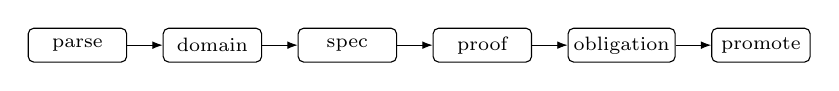
\begin{tikzpicture}[
  node distance=0.45cm,
  box/.style={draw, rounded corners=2pt, align=center, inner sep=2pt,
    minimum width=1.25cm, minimum height=0.43cm, font=\scriptsize},
  arrow/.style={-{Latex[length=1.3mm]}, line width=0.32pt}
]
\node[box] (p) {parse};
\node[box, right=of p] (d) {domain};
\node[box, right=of d] (s) {spec};
\node[box, right=of s] (r) {proof};
\node[box, right=of r] (o) {obligation};
\node[box, right=of o] (m) {promote};
\draw[arrow] (p) -- (d);
\draw[arrow] (d) -- (s);
\draw[arrow] (s) -- (r);
\draw[arrow] (r) -- (o);
\draw[arrow] (o) -- (m);
\end{tikzpicture}
\end{center}
\vspace{-0.7em}
Each gate has a different purpose. Parsing prevents the proposer from escaping
the grammar. Domain checks prevent invalid real logarithms on the bounded
interval. Specification checks compare finite samples. Proof metadata records
whether the current survivor shape is inside the known certificate surface.
Obligation checks connect constructor-plan side conditions to sidecar interval
evidence.

The current bounded regression surface enumerates \(\mathcal{T}_{\le 3}\), a
depth-three EML corpus of 1446 trees, and selects
\[
T^\star
=
\min_{\prec}
\{T\in\mathcal{T}_{\le d}:
\operatorname{err}_{\mathrm{train}}(T,D)\le\varepsilon
\wedge
\operatorname{err}_{\mathrm{holdout}}(T,D)\le\varepsilon\}.
\]
In the checked demo corpus, the selected formulas include the compact
representatives for \(x\), \(\exp(x)\), \(\ln(x)\), and \(\exp(\exp(x))\).
The noisy regression artifact records signed residuals rather than claiming a
general recovery theorem.

\textbf{4. Tau-facing memory update.}
Accepted sidecar evidence is converted into qNS masks and routed through Tau.
The table-memory state is a finite map
\[
M:I\to B_{\mathrm{qNS}}.
\]
The pointwise update is
\[
M_{t+1}(i)
=
\bigl(G(i)\wedge A(i)\bigr)
\vee
\bigl(G(i)'\wedge M_t(i)\bigr).
\]
Standard reading: for each memory slot \(i\), the next memory value is the join
of the replacement value restricted by guard \(G(i)\) and the old memory value
restricted by the prime of \(G(i)\). In the Tau experiment this appears as a
named table-backed revision:
\[
\mathtt{memory\_revise\_qns8(old,guard,replacement)}
\equiv
\mathtt{table\ \{when\ guard => replacement;\ else => old\}}.
\]

\textbf{5. Current executable receipt.}
The public demo path in \texttt{TauLang-Experiments} downloads official Tau,
applies local research patches, builds Tau, and runs the qNS/EML demos. The
current model-free memory fixture reports:
\[
\begin{array}{rcl}
\text{candidate count} &=& 5,\\
\text{parse-ok count} &=& 3,\\
\text{promoted count} &=& 3,\\
\text{review count} &=& 2,\\
\text{memory-updated count} &=& 3,\\
\text{rejected-preserved count} &=& 2.
\end{array}
\]
It also checks that qNS table regressions and symbolic Tau table checks pass.
The important result is not that a language model is trusted. The result is
that model or fixture proposals can enter a narrow evidence pipeline, and only
checked masks can update memory.

\textbf{Boundary.}
The experiment does not prove full symbolic regression, complete EML
normalization, native Tau evaluation of \(\exp\) or \(\ln\), complex
principal-branch correctness, or production safety of an attached LLM. The
mathematical contribution is a scoped architecture:
\[
\operatorname{Proposal}
\to
\operatorname{Grammar}
\to
\operatorname{FiniteChecks}
\to
\operatorname{ProofMetadata}
\to
\operatorname{qNSMasks}
\to
\operatorname{TauGate}
\to
\operatorname{MemoryRevision}.
\]
This is useful because every promotion claim is reducible to finite artifacts
that can be replayed, inspected, and rejected if stale or tampered.

\footnotesize
\textbf{References.}
Andrzej Odrzywolek, ``All elementary functions from a single operator,''
arXiv:2603.21852v2, 2026.
Ohad Asor, \emph{Theories and Applications of Boolean Algebras}, draft v0.25,
2024.
TheDarkLightX, \emph{TauLang-Experiments}, public experiment repository,
\href{https://github.com/TheDarkLightX/TauLang-Experiments}{GitHub}.
Dana Edwards, ``Neuro-symbolic Boolean algebras in Tau Language,'' Tutorial 49,
2026.
Dana Edwards, ``EML trees as neuro-symbolic hypotheses,'' Tutorial 50, 2026.
Dana Edwards, ``Symbolic hypothesis generation with EML and qNS,'' Tutorial 51,
2026.

\end{document}
